\chapter{Introduction to Pattern-Match-Oriented Programming}\label{pmo}

This chapter explains what kind of programming is possible using the syntax for pattern matching and the various built-in patterns introduced in Chapter~\ref{quick}.
To that end, we present frequently occurring patterns in programming that leverages Egison pattern matching.
We hope this chapter gives you a concrete picture of programming with Egison's pattern matching.

\section{List Programming with Pattern Matching}

This section observes how list programming changes with Egison's pattern matching.
Here, by list programming, we mean the kind of programming involved in defining functions typically provided by the list libraries of general programming languages, including functional programming languages.
The join pattern \lstinline{_ ++ $x :: _}, whose second argument is a cons pattern, appears frequently in list programming.
For this reason, we have given this pattern a name and call it the \emph{join-cons pattern}.
As this section shows, many functions on lists can be defined using the join-cons pattern.

\subsection{A Single Join-Cons Pattern --- the \texttt{map} Function and Its Relatives}

For the \lstinline{list} matcher, the pattern \lstinline|_ ++ $x :: _| matches each element of the target.
As a result, the following \lstinline{matchAll} expression matches each element of \lstinline{xs} and returns the result of applying the function \lstinline{f} to each of them.
This is precisely the definition of the \lstinline{map} function.
The type annotation indicates that the \lstinline{map} function takes a list of an arbitrary type \lstinline{a} and returns a list of type \lstinline{b}.

\begin{lstlisting}[language=egison,numbers=none]
def map (f: a -> b) (xs: [a]) : [b] := matchAll xs as list something with
  | _ ++ $x :: _ -> f x
\end{lstlisting}

By modifying this \lstinline{matchAll} expression, we can define various functions.
For example, the \lstinline{filter} function can be defined by inserting a predicate pattern.
The type annotation indicates that the predicate function \lstinline{pred} takes a value of type \lstinline{a} and returns a \lstinline{Bool}.

\begin{lstlisting}[language=egison,numbers=none]
def filter (pred: a -> Bool) (xs: [a]) : [a] := matchAll xs as list something with
  | _ ++ (?pred & $x) :: _ -> x
\end{lstlisting}

The \lstinline{member} function can be defined by inserting a value pattern.
The \lstinline{member} function is a predicate that determines whether the first argument is contained in the collection given as the second argument.
The \lstinline{member} function is defined using a \lstinline{match} expression.
The \lstinline{match} expression is implemented as an alias for \lstinline{car (matchAll ...)}\footnote{\lstinline{car} is a function that extracts the first element of a collection.}.
This implementation is possible because Egison lazily evaluates \lstinline{matchAll} expressions.
%\footnote{\lstinline{matchAll} also can handle multiple match clauses. \lstinline{matchAll} $t$ \lstinline{as} $m$ \lstinline{with} $c_1$ $c_2$ $...$ is equivalent to \lstinline{matchAll} $t$ \lstinline{as} $m$ \lstinline{with} $c_1$ \lstinline{++} \lstinline{matchAll} $t$ \lstinline{as} $m$ \lstinline{with} $c_2$ \lstinline{++} $...$.}
The type annotation indicates that the \lstinline{member} function takes a value and a list of an arbitrary type \lstinline{a} and returns a \lstinline{Bool}.

{\footnotesize
\begin{lstlisting}[language=egison,numbers=none]
def member (x: a) (xs: [a]) : Bool := match xs as list eq with
  | _ ++ #x :: _ -> True
  | _            -> False
\end{lstlisting}
}

The \lstinline{delete} function can be implemented by slightly modifying the \lstinline{member} function.
The \lstinline{delete} function removes the first occurrence of the first argument \lstinline{x} from the collection \lstinline{xs} given as the second argument.

{\footnotesize
\begin{lstlisting}[language=egison,numbers=none]
def delete (x: a) (xs: [a]) : [a] := match xs as list eq with
  | $hs ++ #x :: $ts -> hs ++ ts
  | _                -> xs
\end{lstlisting}
}

The predicates \lstinline{any} and \lstinline{every} can similarly be implemented using \lstinline{match} expressions.
\lstinline{any} is a predicate that determines whether any element in the collection given as the second argument satisfies the predicate given as the first argument.
\lstinline{every} is a predicate that determines whether all elements in the collection given as the second argument satisfy the predicate given as the first argument.

\begin{lstlisting}[language=egison,numbers=none]
def any (pred: a -> Bool) (xs: [a]) : Bool := match xs as list something with
  | _ ++ ?pred :: _ -> True
  | _               -> False

def every (pred: a -> Bool) (xs: [a]) : Bool := match xs as list something with
  | _ ++ !?pred :: _ -> False
  | _                -> True
\end{lstlisting}

\subsection{Nesting Join-Cons Patterns --- the \texttt{unique} and \texttt{concat} Functions}\label{pmo-nested-join-cons}

By combining multiple join-cons patterns, we can create even more powerful patterns.
As an example, we introduce the \lstinline{unique} function.
When the \lstinline{unique} function is defined using pattern-match-oriented programming, it looks as follows.
The type annotation indicates that the \lstinline{unique} function takes a list of an arbitrary type \lstinline{a} and returns a list of the same type.
\begin{lstlisting}[language=egison,numbers=none]
def unique (xs: [a]) : [a] := matchAllDFS xs as list eq with
  | _ ++ $x :: !(_ ++ #x :: _) -> x
\end{lstlisting}
The not pattern is used to express that \lstinline{x} does \emph{not} appear any further after itself.
As a result, this pattern matches the last occurrence of each element.
\begin{lstlisting}[language=egison,numbers=none]
unique [1,2,3,2,4] -- [1,3,2,4]
\end{lstlisting}

It is also possible to define a \lstinline{unique} function that returns a collection consisting of the first occurrence of each element by making good use of predicate patterns.
To match only the first occurrence, we need to write a pattern that matches when the same element does not appear before that element.
Because Egison's pattern matching processes patterns from left to right, such a pattern cannot be written by simply combining cons patterns and join patterns.
\begin{lstlisting}[language=egison,numbers=none]
def unique2 (xs: [a]) : [a] := matchAllDFS xs as list eq with
  | $hs ++ (!?(\x -> member x hs) & $x) :: _ -> x

unique2 [1,2,3,2,4] -- [1,2,3,4]
\end{lstlisting}

Another more elegant approach is to use sequential patterns.
The same pattern can be expressed using a sequential pattern with a deferred pattern variable in the first argument of the join pattern.
\begin{lstlisting}[language=egison,numbers=none]
def unique (xs: [a]) : [a] := matchAllDFS xs as list eq with
  |  {@               ++ $x :: _,
      !(_ ++ #x :: _)}
  -> x
\end{lstlisting}

Another example of nested join-cons patterns is the \lstinline{concat} function introduced in Section~\ref{quick-matchalldfs} of Chapter~\ref{quick}.
By combining matcher composition (Section~\ref{quick-matcher-composition} of Chapter~\ref{quick}) with the join-cons pattern, we can define \lstinline{concat} using pattern-match-oriented programming.
The type annotation indicates that the \lstinline{concat} function takes a list of lists and returns a flattened list.
\begin{lstlisting}[language=egison,numbers=none]
def concat (xss: [[a]]) : [a] := matchAllDFS xss as list (list something) with
  | _ ++ (_ ++ $x :: _) :: _ -> x
\end{lstlisting}


\section{Multiset Programming}

The ability to directly pattern-match on multisets is a major feature of Egison.
This section introduces techniques for programming that takes advantage of multiset pattern matching.
From this point on, nearly all pattern matching in this book involves multiset pattern matching.

\subsection{Cons Patterns on Multisets}

The cons pattern of the \lstinline{multiset} matcher is useful for pattern matching on collections while ignoring the order of elements.
Such situations frequently arise when describing mathematical algorithms.

Let us start with a simple example.
The \lstinline{lookup} function on association lists can be defined with a single cons pattern.
A single multiset cons pattern can also be replaced with a list join-cons pattern.
The type annotation indicates that the \lstinline{lookup} function takes a key \lstinline{k} and an association list and returns the corresponding value.
\begin{lstlisting}[language=egison,numbers=none]
def lookup (k: a) (ls: [(a, b)]) : b := match ls as multiset (eq, something) with
  | (#k, $x) :: _ -> x
\end{lstlisting}
However, nested multiset cons patterns cannot be replaced with list join-cons patterns.
A $k$-fold nested multiset cons pattern can be used to enumerate $P(n,k) = \frac{n!}{(n-k)!}$ permutations of $k$ elements, whereas a $k$-fold nested list join-cons pattern can be used to enumerate $C(n,k) = \frac{n!}{k!(n-k)!}$ combinations of $k$ elements.
\begin{lstlisting}[language=egison,numbers=none]
matchAll [1, 2, 3] as list something with
| _ ++ $x :: _ ++ $y :: _ -> (x, y)
-- [(1,2),(1,3),(2,3)]

matchAll [1, 2, 3] as multiset something with
| $x :: $y :: _ -> (x, y)
-- [(1,2),(1,3),(2,1),(2,3),(3,1),(3,2)]
\end{lstlisting}
An equivalent program can be written in traditional functional programming using list comprehensions as follows.
\lstinline{tails} is a function that returns the suffixes of the argument list.
\lstinline{splits} is a function that decomposes the argument list into a prefix and the remaining list.
\begin{lstlisting}[language=egison,numbers=none]
[ (x, y) | x : ts <- tails [1, 2, 3], y <- ts ]
-- [(1,2),(1,3),(2,3)]

[ (x, y) | (hs, x : ts) <- splits [1, 2, 3], y <- hs ++ ts ]
-- [(1,2),(1,3),(2,1),(2,3),(3,1),(3,2)]
\end{lstlisting}

Although traditional programming languages also provide libraries for multisets, there are many situations where collections that one wants to treat as multisets must be reconsidered as lists.
In fact, in the enumeration of $C(n,2)$ combinations using list comprehensions above, two list-processing functions---\lstinline{splits} and \lstinline{++}---are used, describing processing that reconsiders the target collection as a list.
Pattern matching on multisets hides such list-based reconversion inside the pattern definition (in this case, the definition of the \lstinline{::} pattern of the \lstinline{multiset} matcher), thereby broadening the opportunities to directly treat collections that one wants to handle as multisets.
The remainder of this book describes various patterns on multisets, combined with the patterns introduced in Chapter~\ref{quick}.


\subsection{Poker Hand Evaluation}\label{pmo-poker}

As an application of non-linear patterns on multisets, we present poker hand evaluation.
Using non-linear patterns on multisets, every poker hand can be expressed as a single pattern.
\footnote{When the author designed Egison's match expressions, the ability to concisely write a program for poker hand evaluation was one of the design requirements.}
The pattern ``\lstinline{[}$p_1$\lstinline{,} $p_2$\lstinline{,} $...$\lstinline{,} $p_n$\lstinline{]}'' is syntactic sugar that expands to ``$p1$ \lstinline{:} $p_2$ \lstinline{:} $...$ \lstinline{:} $p_n$ \lstinline{: []}''.
\begin{lstlisting}[language=egison,numbers=none]
def poker (cs: [Card]) : String :=
  match cs as multiset card with
  | card $s $n :: card #s #(n-1) :: card #s #(n-2) :: card #s #(n-3) :: card #s #(n-4) :: _
    -> "Straight flush"
  | card _ $n :: card _ #n :: card _ #n :: card _ #n :: _ :: []
    -> "Four of a kind"
  | card _ $m :: card _ #m :: card _ #m :: card _ $n :: card _ #n :: []
    -> "Full house"
  | card $s _ :: card #s _ :: card #s _ :: card #s _ :: card #s _ :: []
    -> "Flush"
  | card _ $n :: card _ #(n-1) :: card _ #(n-2) :: card _ #(n-3) :: card _ #(n-4) :: []
    -> "Straight"
  | card _ $n :: card _ #n :: card _ #n :: _ :: _ :: []
    -> "Three of a kind"
  | card _ $m :: card _ #m :: card _ $n :: card _ #n :: _ :: []
    -> "Two pair"
  | card _ $n :: card _ #n :: _ :: _ :: _ :: []
    -> "One pair"
  | _ :: _ :: _ :: _ :: _ :: [] -> "Nothing"
\end{lstlisting}
This \lstinline{poker} function works as follows.
\begin{lstlisting}[language=egison,numbers=none]
poker [Card Spade 5, Card Spade 6, Card Spade 7, Card Spade 8, Card Spade 9]
-- "Straight flush"
poker [Card Spade 5, Card Diamond 5, Card Spade 7, Card Club 5, Card Heart 5]
-- "Four of a kind"
poker [Card Spade 5, Card Diamond 5, Card Spade 7, Card Club 5, Card Heart 7]
-- "Full house"
poker [Card Spade 5, Card Spade 6, Card Spade 7, Card Spade 13, Card Spade 9]
-- "Flush"
poker [Card Spade 5, Card Club 6, Card Spade 7, Card Spade 8, Card Spade 9]
-- "Straight"
poker [Card Spade 5, Card Diamond 5, Card Spade 7, Card Club 5, Card Heart 8]
-- "Three of a kind"
poker [Card Spade 5, Card Diamond 10, Card Spade 7, Card Club 5, Card Heart 10]
-- "Two pair"
poker [Card Spade 5, Card Diamond 10, Card Spade 7, Card Club 5, Card Heart 8]
-- "One pair"
poker [Card Spade 5, Card Spade 6, Card Spade 7, Card Spade 8, Card Diamond 11]
-- "Nothing"
\end{lstlisting}
Egison has a rule that pattern constructors (such as \lstinline{card}) begin with a lowercase letter, while data constructors (such as \lstinline{Card}) begin with an uppercase letter.
The type annotation of the \lstinline{poker} function indicates that it takes a list of cards and returns a string representing the hand.

Note that in the above example, the card matcher is defined as an algebraic data matcher as follows.
\begin{lstlisting}[language=egison,numbers=none]
def suit := algebraicDataMatcher
  | spade
  | heart
  | club
  | diamond

def card := algebraicDataMatcher
  | card suit (mod 13)
\end{lstlisting}

\section{Comparing Data with Tuple Patterns}\label{pmo-tuple}

Situations where one wants to compare multiple pieces of data arise frequently in programming.
In such situations, tuple patterns, especially when used together with not patterns, are often useful.
For example, the \lstinline{difference} function can be defined by inserting a not pattern into the implementation of the \lstinline{intersect} function introduced in Section~\ref{quick-matcher-composition} of Chapter~\ref{quick}.
The type annotation indicates that the function takes two sets and returns their difference.
\begin{lstlisting}[language=egison,numbers=none]
def difference (xs: [a]) (ys: [a]) : [a] := matchAll (xs, ys) as (set eq, set eq) with
  | ($x :: _, !(#x :: _)) -> x
\end{lstlisting}
By changing the insertion position of the not pattern to \lstinline|!($x :: _, #x :: _)|, we can also write a pattern that succeeds when the two collections have no common elements at all.

By combining these patterns with sequential patterns, we can write even more complex patterns.
This is because sequential patterns make it possible to apply a not pattern collectively to multiple separate parts of a pattern.
For example, in Section~\ref{quick-seq-pat} of Chapter~\ref{quick}, we defined the \lstinline{singleCommonElem} function, which checks whether two collections have exactly one common element, using pattern matching.
Sequential not patterns sometimes become necessary when describing mathematical algorithms.
For instance, sequential not patterns also appear in the SAT solver implementation introduced in Section~\ref{essence-sat} of Chapter~\ref{essence}.
The type annotation indicates that the function takes two lists and returns a boolean.
\begin{lstlisting}[language=egison,numbers=none]
def singleCommonElem (xs: [a]) (ys: [a]) : Bool := match (xs, ys) as (multiset eq, multiset eq) with
                    | [($x :: @, #x :: @),
                       !($y :: _, #y :: _)] -> True
                    | _ -> False
\end{lstlisting}

It is also possible to combine sequential patterns with loop patterns.
For example, a pattern that matches the common prefix of two lists can be written using a sequential loop pattern.
\begin{lstlisting}[language=egison,numbers=none]
match (xs, ys) as (list eq, list eq) with
| loop $i (1,$n)
    [($x_i :: @, #x_i :: @), [...]]
    !($y :: _, #y :: _)
-> map (\i -> x_i) [1..n]
\end{lstlisting}

\section{Recursive Patterns with Loop Patterns}\label{pmo-loop}

Loop patterns are used to express repetition of patterns.
Loop patterns are useful for constructing complex patterns by combining simple pattern constructors, or for writing patterns in which the number of pattern variables depends on a parameter.
In such situations, complex recursion needs to be written.
With loop patterns, such recursion can be pushed into the pattern, enabling intuitive descriptions.
This section presents such examples.

\subsection{The N-Queens Problem}\label{pmo-loop-nqueen}

This section introduces a technically sophisticated yet tricky example of loop patterns by presenting a program that solves the N-Queens problem.
The N-Queens problem is the problem of placing $n$ chess queens on an $n \times n$ chessboard so that no two queens threaten each other.
A chess queen can attack any piece that is any number of squares away horizontally, vertically, or diagonally.
In terms of Japanese chess (shogi), the queen combines the moves of the rook and the bishop.

Let us start with a program that solves the $4$-Queens problem.
In this program, the placement of the $4$ queens is represented as a list.
The $n$-th element of the list represents which column the queen in the $n$-th row is placed in.
In this case, the solution must be a permutation of the elements of the collection \lstinline|[1,2,3,4]|,
because no two queens can be placed in the same row or column.
Therefore, we pattern-match the collection \lstinline|[1,2,3,4]| as a multiset of integers.
The condition that queens cannot share a diagonal line is expressed by the conditions $a_1 \pm 1 \neq a_2$, $a_1 \pm 2 \neq a_3$, $a_2 \pm 1 \neq a_3$, $a_1 \pm 3 \neq a_4$, $a_2 \pm 2 \neq a_4$, and $a_3 \pm 1 \neq a_4$.
\begin{lstlisting}[language=egison,numbers=none]
matchAll [1,2,3,4] as multiset integer with
  $a_1 ::
   (!#(a_1 - 1) & !#(a_1 + 1) & $a_2) ::
    (!#(a_1 - 2) & !#(a_1 + 2) & !#(a_2 - 1) & !#(a_2 + 1) & $a_3) ::
     (!#(a_1 - 3) & !#(a_1 + 3) & !#(a_2 - 2) & !#(a_2 + 2) & !#(a_3 - 1) & !#(a_3 + 1) & $a_4) ::
      [] -> [a_1,a_2,a_3,a_4]
-- [[2,4,1,3],[3,1,4,2]]
\end{lstlisting}
To generalize the above program for the $n$-Queens problem, doubly nested loop patterns can be used.
The index variable \lstinline|i| of the outer loop pattern is used in the index range of the inner loop pattern to express the difference in the number of repetitions of the inner loop.
Also note that values bound in previous repetition patterns, for example the value bound to \lstinline|$a_j|, are referenced as in \lstinline|#(a_j - (i - j))| and \lstinline|#(a_j + (i - j))|.
In this way, the non-linearity of indexed pattern variables (the ability to reference values bound to indexed pattern variables on the left side of the pattern) works effectively.
The type annotation indicates that the \lstinline{nQueens} function takes an integer \lstinline{n} and returns a list of lists of integers.
\begin{lstlisting}[language=egison,numbers=none]
def nQueens (n: Integer) : [[Integer]] :=
  matchAll [1..n] as multiset integer with
  | $a_1 ::
     (loop $i (2,n)
           ((loop $j (1, i - 1)
                  (!#(a_j - (i - j)) & !#(a_j + (i - j)) & ...)
                  $a_i) :: ...)
           [] -> map (\i -> a_i) [1..n]

nQueens 4 -- [[2,4,1,3],[3,1,4,2]]
\end{lstlisting}

\subsection{Pattern Matching on Trees}\label{pmo-tree}

This section introduces a practical example of loop patterns by demonstrating pattern matching on trees.
The tree nodes in this section can have an arbitrary number of subtrees as children, similar to XML.
Furthermore, these subtrees are treated as multisets.
A matcher for such trees was defined in Section~\ref{quick-matcher-composition} of Chapter~\ref{quick}.
We use that matcher in this section.

We write patterns against a tree that categorizes programming languages.
\lstinline{treeData} defines that category tree.
For example, \lstinline{"Egison"} belongs to the \lstinline{"pattern-match-oriented"} category and to the \lstinline{"Dynamically typed"} subcategory of the \lstinline{"Functional language"} category.
Data constructors \lstinline{Node} and \lstinline{Leaf} begin with uppercase letters.
\begin{lstlisting}[language=egison,numbers=none]
def treeData :=
  Node "Programming language"
    [Node "pattern-match-oriented" [Leaf "Egison"],
     Node "Functional language"
       [Node "Strictly typed" [Leaf "OCaml", Leaf "Haskell", Leaf "Curry", Leaf "Coq"],
        Node "Dynamically typed" [Leaf "Egison", Leaf "Lisp", Leaf "Scheme", Leaf "Racket"]],
     Node "Logic programming" [Leaf "Prolog", Leaf "Curry"],
     Node "Object oriented" [Leaf "C++", Leaf "Java", Leaf "Ruby", Leaf "Python", Leaf "OCaml"]]
\end{lstlisting}

The following \lstinline{matchAll} expression enumerates the categories to which a given language belongs.
Because a leaf of the tree can be at any depth, a loop pattern whose index range end value is a pattern (in this case \lstinline{$n}) is used.
The ellipsis pattern of this loop pattern is positioned not at the end of the repetition pattern.
The ability for users to specify the position of repetition is another strength of loop patterns that the Kleene star operator of regular expressions does not have.
Pattern constructors \lstinline{node} and \lstinline{leaf} begin with lowercase letters.
The type annotation indicates that the \lstinline{ancestors} function takes a string \lstinline{x} and a tree \lstinline{t} and returns a list of ancestor node paths.
\begin{lstlisting}[language=egison,numbers=none]
def ancestors (x: String) (t: Tree String) : [[String]] := matchAll t as tree string with
  | loop $i (1,$n)
      (node $c_i (... ::  _))
      (leaf #x)
  -> map (\i -> c_i) [1..n]

ancestors "Egison" treeData
-- [["Programming language", "pattern-match-oriented"], ["Programming language", "Functional language", "Dynamically typed"]]
\end{lstlisting}

It is also possible to write a pattern that enumerates all languages belonging to a given subcategory.
By using doubly nested loop patterns, the subcategory can be at any depth.
The following pattern enumerates all languages belonging to a specific category.
\lstinline{matchAllDFS} is used to enumerate languages in the same order as they appear in the tree.
The type annotation indicates that the \lstinline{descendants} function takes a string \lstinline{x} and a tree \lstinline{t} and returns a list of descendant nodes.
\begin{lstlisting}[language=egison,numbers=none]
def descendants (x: String) (t: Tree String) : [String] := matchAllDFS t as tree string with
  | loop _ (1,_)
      (node _ (... ::  _))
      (node #x ((loop _ (1,_)
                   (node _ (... :: _))
                   (leaf $y)) :: _))
  -> y

descendants "Functional language" treeData
-- ["OCaml", "Haskell", "Curry", "Coq", "Egison", "Lisp", "Scheme", "Racket"]
\end{lstlisting}

A DSL (domain-specific language) capable of pattern matching on trees is XML Path.
An advantage of Egison is that a wide variety of patterns can be described by combining a small number of user-definable pattern constructors with loop patterns.
XML Path, by contrast, uses many built-in commands such as the \lstinline{ancestor} command to describe patterns.

\subsection{Pattern Matching on Graphs}\label{pmo-graph}

This section introduces pattern matching on graphs.
We present pattern matching on both graphs represented as sets of edges and graphs represented as adjacency lists.

\subsubsection{Graphs as Sets of Edges}\label{pmo-graph-set}

This section performs pattern matching on graphs represented as sets of edges.
First, we define the following matcher and graph.
\begin{lstlisting}[language=egison,numbers=none]
def graph := set edge
def edge := algebraicDataMatcher
  | edge integer integer

def graphData :=
  [ Edge 1 2, Edge 2 1, Edge 2 3,  Edge 2 4, Edge 3 4, Edge 4 5, Edge 4 6, Edge 4 7
  , Edge 5 4, Edge 5 6, Edge 5 7,  Edge 6 4, Edge 6 5, Edge 6 7, Edge 7 4, Edge 7 5
  , Edge 7 6, Edge 7 8, Edge 9 10, Edge 10 7 ]
\end{lstlisting}
\begin{figure}[t]
  \centering
  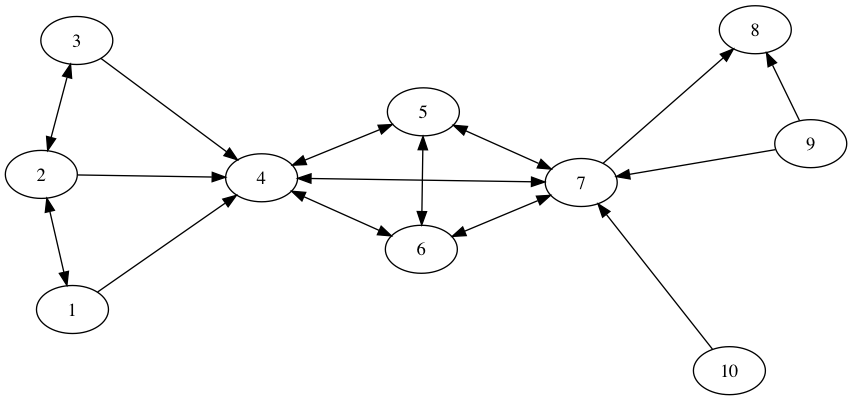
\includegraphics[width=12cm,bb=0 0 852 400]{graph.png}
  \caption{Visualization of \lstinline{graphData}}
  \label{fig:graphVis}
\end{figure}
The pattern constructor \lstinline{edge} begins with a lowercase letter, while the data constructor \lstinline{Edge} begins with an uppercase letter.
Figure~\ref{fig:graphVis} shows a visualization of the above graph.
This section presents several pattern matches on this graph.

A pattern that enumerates all nodes reachable from a given node \lstinline{s} by traversing two edges can be written as follows.
\begin{lstlisting}[language=egison,numbers=none]
let s := 1 in
  matchAll graphData as graph with
  | edge (#s & $x_1) $x_2 :: edge #x_2 $x_3 :: _
  -> x
-- [1,3,4,5,6,7]
\end{lstlisting}
A pattern that enumerates nodes connected to node \lstinline{s} via an edge originating from \lstinline{s}, but which do not themselves have an edge back to \lstinline{s}, can be written using a not pattern as follows.
\begin{lstlisting}[language=egison,numbers=none]
let s := 1 in
  matchAll graphData as graph with
  | edge #s $x :: !(edge #x #s :: _)
  -> x
-- [4]
\end{lstlisting}
A pattern that enumerates all paths from node \lstinline{s} to node \lstinline{e} can be written using a loop pattern.
Egison allows the use of \lstinline{let} expressions within patterns.
This \lstinline{let} expression is used to bind \lstinline{s} to \lstinline{$x_1}.
Thanks to this \lstinline{let} expression, the first repetition of the loop pattern does not need to be treated as a special case.
\begin{lstlisting}[language=egison,numbers=none]
let (s, e) := (1, 8) in
  matchAll graphData as graph with
  | let x_1 := s in
      loop $i (2, $n)
           (edge #x_(i - 1) $x_i :: ...)
           (edge #x_(n - 1) (#e & $x_n) :: _)
  -> map (\i -> x_i) [1..n]
-- [[1,4,7,8], ...]
\end{lstlisting}
A pattern that enumerates cliques (subgraphs forming complete graphs) of size $n$ can be written as follows.
It uses doubly nested loop patterns.
\begin{lstlisting}[language=egison,numbers=none]
let n := 4 in
  matchAll graphData2 as graph with
  | edge $x_1 $x_2 :: loop $i (3, n)
                           (edge #x_1 $x_i :: loop $j (2, i - 1)
                                                   (edge #x_j #x_i :: ...)
                                                   ...)
                          _
  -> map (\i -> x_i) [1..n]
-- [[4,5,6,7],...]
\end{lstlisting}

This section presented pattern matching on directed graphs.
It is straightforward to modify the above patterns for directed graphs into patterns for undirected graphs: simply use a matcher that identifies \lstinline{Edge a b} and \lstinline{Edge b a}.
Such a matcher for undirected graphs can be defined using the matcher for unordered pairs introduced in Section~\ref{matcher-basic} of Chapter~\ref{matcher}.

\subsubsection{Adjacency Graphs}

This section performs pattern matching on graphs represented as weighted adjacency lists.
A matcher for weighted adjacency lists can be defined using matcher composition (Section~\ref{quick-matcher-composition} of Chapter~\ref{quick}).
The \lstinline{graphData} in the program below represents a network of cities connected by air routes as a weighted adjacency list.
The travel time between two cities is represented as an integer weight.
\begin{lstlisting}[language=egison,numbers=none]
def graph := multiset (string, multiset (string, integer))

def graphData :=
  [("Berlin", [("New York", 14), ("London", 2), ("Tokyo", 14), ("Vancouver", 13)]),
   ("New York", [("Berlin", 14), ("London", 12), ("Tokyo", 18), ("Vancouver", 6)]),
   ("London", [("Berlin", 2), ("New York", 12), ("Tokyo", 15), ("Vancouver", 10)]),
   ("Tokyo", [("Berlin", 14), ("New York", 18), ("London", 15), ("Vancouver", 12)]),
   ("Vancouver", [("Berlin", 13), ("New York", 6), ("London", 10), ("Tokyo", 12)])]
\end{lstlisting}
The pattern in the following program matches routes that depart from Berlin, visit all cities, and return to Berlin.
This pattern is used to solve the traveling salesman problem.
It makes effective use of non-linear loop patterns.
The type annotation indicates that the \lstinline{trips} function computes a list of routes from the graph data and returns a list of tuples of total distance and city list.
\begin{lstlisting}[language=egison,numbers=none]
def trips : [(Integer, [String])] :=
  let n := length graphData in
    matchAll graphData as graph with
    | (#"Berlin", (($s_1,$p_1) :: _)) ::
        loop $i (2, n - 1)
          ((#s_(i - 1), ($s_i, $p_i) :: _) :: ...)
          ((#s_(n - 1), (#"Berlin" & $s_n, $p_n) :: _) :: [])
    -> (sum (map (\i -> p_i) [1..n]), map (\i -> s_i) [1..n])

head (sortBy (\(_, x), (_, y) -> compare x y) trips)
-- (46, ["London", "New York", "Vancouver", "Tokyo", "Berlin"])
\end{lstlisting}

As with trees (Section~\ref{pmo-tree}), several DSLs for pattern matching on graphs have been developed as query languages for graph databases.
An advantage of Egison over these DSLs is that a wide variety of patterns can be expressed by combining a small number of user-defined pattern constructors with a few built-in patterns, including loop patterns.
